\chapter{Working with Raster Data}
QGIS supports a number of raster data formats. This section describes how to work with raster data in QGIS.
\section{What is raster data?}
index{rasters!definition}
Raster data in GIS are matrices of discrete cells that represent features on, above or below the earth's surface. Each cell in the raster grid is the same size, and cells are usually rectangular (in QGIS they will always be rectangular). Typical raster datasets include remote sensing data such as aerial photography or satellite imagery and modelled data such as an elevation matrix.

Unlike vector data, raster data typically do not have an associated database record for each cell.

In GIS, a raster layer would have georeferencing data associated with it which
will allow it to be positioned correctly in the map display to allow other
vector and raster data to be overlaid with it. QGIS makes use of georeferenced
rasters to properly display the data.\index{rasters!georeferenced}
	
\section{Raster formats supported in QGIS}
QGIS supports a number of different raster formats. Currently tested formats
include:\index{rasters!formats}
\begin{compactitem}
\item Arc/Info Binary Grid
\item Arc/Info ASCII Grid
\item Grass Raster
\item GeoTIFF
\item Spatial Data Transfer Standard Grids (with some limitations)
\item USGS ASCII DEM
\item Erdas Imagine
\end{compactitem}
Because the raster implementation in QGIS is based on the GDAL library, other
raster formats implemented in GDAL are also likely to work, but have not yet
been tested. See Appendix \ref{appdx_gdal} for more
details.\index{rasters!implementation}
	
\section{Loading raster data in QGIS}
\parpic[l]{
\includegraphics{qgis_user_guide_images/addraster}}Raster layers are
loaded either by clicking on the Load Raster icon or by selecting the View->Add
Raster Layer menu option. More than one layer can be loaded at the same time by
holding down the Control key and clicking on multiple items in the file
dialog.\index{rasters!loading}
	
\section{Raster Properties}

\parpic[r]{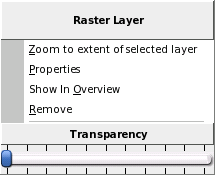
\includegraphics[scale=0.6]{qgis_user_guide_images/rastercontextmenu}}To
view and set the properties for a raster layer, right click on the layer name.
This displays the raster layer context menu that includes a number of items that
allow you to:\index{rasters!context menu}
\begin{compactitem}
\item Zoom to the full extent of the raster
\item Show the raster in the map overview window
\item Open the properties dialog (of course)
\item Remove the layer from the map
\item Set the transparency using a slider control
\end{compactitem}
Choose \textsl{Properties} from the context menu to open the raster properties
dialog for the layer.\index{rasters!properties}


Figure \ref{fig:raster_properties} shows the properties dialog. There are four tabs on the dialog: \textsl{Symbology}, \textsl{General}, \textsl{Metadata}, and \textsl{Pyramids}.

\begin{figure}[h]
   \begin{center}
   \caption{Raster Layers Properties Dialog}\label{fig:raster_properties}\smallskip
   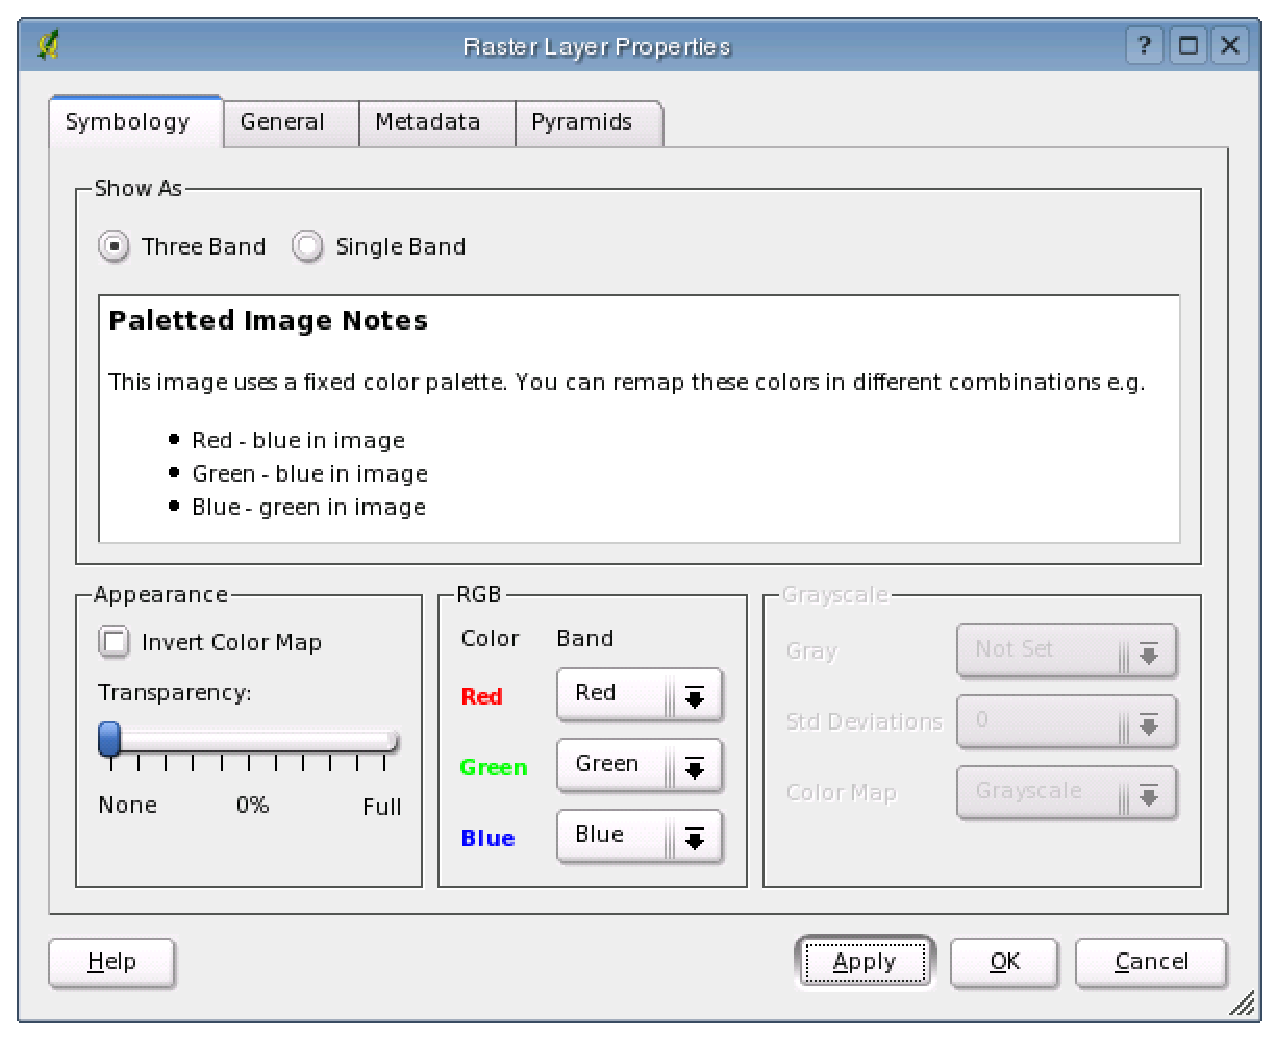
\includegraphics[scale=.7]{qgis_user_guide_images/raster_properties}
\end{center}  
\end{figure}


\subsection{Symbology Tab}


QGIS supports three forms of raster layers:\index{rasters!supported forms}
\begin{compactitem}
\item Single Band Grayscale Rasters
\item Palette Based RGB Rasters
\item Multiband RGB Rasters
\end{compactitem}

From these three basic layer types, eight forms of symbolised raster display can
be used:\index{rasters!renderers}
\begin{compactenum}

\item Single Band Grayscale
\item Single Band Pseudocolor
\item Paletted Grayscale (where only the red, green or blue component of the image is displayed)
\item Paletted Pseudocolor (where only the red, green or blue component of the image is displayed, but using a pseudocolor algorithm)
\item Paletted RGB
\item Multiband Grayscale (using only one of the bands to display the image)
\item Mulitiband Pseudocolor (using only one of the bands shown in pseudocolor)
\item Multiband RGB (using any combination of three bands)
\end{compactenum}
\smallskip
QGIS can invert the colors in a given layer so that light colors become dark
(and dark colors become light). Use the \textsl{Invert Color Map} checkbox to
enable / disable this behavior.\index{rasters!inverting the color map}

QGIS has the ability to display each raster layer at varying transparency
levels.\index{rasters!transparency} Use the transparency slider to indicate to what extent the underlying layers (if any) should be visible though the current raster layer. The transparency can also be set using the transparency slider in the layer context menu which is accessible by right-clicking on the layer in the legend.

QGIS can restrict the data displayed to only show cells whose values are within
a given number of standard deviations of the mean for the
layer.\index{rasters!standard deviation} This is useful when you have one or two cells with abnormally high values in a raster grid that are having a negative impact on the rendering of the raster. This option is only available for pseudocolor images.

\subsection{General Tab}
The General tab displays basic information about the selected raster, including
the layer source and  display name in the legend (which can be modified). This
tab also shows a thumbnail of the layer, its legend symbol, and the
palette.\index{rasters!properties}

\subsection{Metadata Tab}
The Metadata tab displays a wealth of information about the raster layer,
including statistics about each band in the current raster layer. Statistics are
gathered on a 'need to know' basis, so it may well be that a given layers
statistics have not yet been collected.\index{rasters!metadata}


\begin{Tip}\caption{\textsc{Gathering Raster Statistics}}
\qgistip{To gather statistics for a layer, select pseudocolor rendering and
click the \textsl{Apply} button. Gathering statistics for a layer can be time
consuming. Please be patient while QGIS examines your
data!\index{rasters!statistics}
}
\end{Tip}
\subsection{Pyramids Tab}
\label{raster_pyramids}
Large resolution raster layers can slow navigation in QGIS. By creating lower
resolution copies of the data (pyramids), performance can be considerably
improved as QGIS selects the most suitable resolution to use depending on the
level of zoom.\index{rasters!building pyramids} 

You must have write access in the directory where the original data is stored to build pyramids. 

Please note that building pyramids may alter the original data file and once created they cannot be removed. If you wish to preserve a 'non-pyramided' version of your raster, make a backup copy prior to building pyramids.
